%                                                                 aa.dem
% AA vers. 8.2, LaTeX class for Astronomy & Astrophysics
% demonstration file
%                                                       (c) EDP Sciences
%-----------------------------------------------------------------------
%
%\documentclass[referee]{aa} % for a referee version
%\documentclass[onecolumn]{aa} % for a paper on 1 column  
%\documentclass[longauth]{aa} % for the long lists of affiliations 
%\documentclass[rnote]{aa} % for the research notes
%\documentclass[letter]{aa} % for the letters 
%\documentclass[bibyear]{aa} % if the references are not structured 
% according to the author-year natbib style

%%%%%%%%%%%%%%%%%%%%%%%%%%%%%%%%%%%%%%%%%%%%%%%%%%%%%%%%%%%%%%%%%%%%%%%%%%%%
\documentclass{aa}    %% Astronomy & Astrophysics style class aa.cls v8.2
%\documentclass[referee]{aa} 

\usepackage{graphicx,url,twoopt,natbib}
\usepackage[varg]{txfonts}           %% A&A font choice

\usepackage{pdfcomment}              %% for popup acronym meanings
\usepackage{acronym}                 %% for popup acronym meanings

\usepackage{url}
\usepackage{color,hyperref}
\definecolor{linkcolor}{rgb}{0,0.3,0.7}
\hypersetup{colorlinks=true,
	linkcolor=linkcolor, 
	citecolor=linkcolor,
	filecolor=linkcolor, 
	urlcolor=linkcolor}

\usepackage{natbib}

\bibpunct{(}{)}{,}{a}{}{,}    %% natbib cite format used by A&A and ApJ

% Manually specified definitions
\input{definitions.tex}

\usepackage{xcolor}
\newcommand\todo[1]{\textbf{(#1)}}

\begin{document}
	
\title{The host galaxy of the short GRB~111117A at $z = 2.211$\thanks{Based on observations collected at the European Southern Observatory, Paranal, Chile, Program ID: 088.A-0051 and 091.D-0904.}}

\titlerunning{GRB~111117A}


\author{J.~Selsing\inst{1}
\and T.~Kr\"{u}hler\inst{2}
\and D.~Malesani\inst{1,3}
\and P.~D'Avanzo\inst{4}
\and J.~Palmerio\inst{5}
\and S.~D.~Vergani\inst{6}
\and J.~Japelj\inst{7}
\and B.~Milvang-Jensen\inst{1}
\and D.~Watson\inst{1}
\and P.~Jakobsson\inst{8}
%
\and Z.~Cano\inst{9}
%\and L.~B.~Christensen\inst{1}
\and V.~D'Elia\inst{10}
\and A.~de~Ugarte~Postigo\inst{9, 1}
\and J.~P.~U.~Fynbo\inst{1}
\and A.~Gomboc\inst{11}
\and K.~E.~Heintz\inst{8,1}
\and A.~J.~Levan \inst{12}
\and S.~Schulze \inst{13, 14}
\and M.~Sparre\inst{1,15}
\and N.~R.~Tanvir\inst{16}
\and C.~C.~Th\"one\inst{9}
}


\institute{Dark Cosmology Centre, Niels Bohr Institute, University of Copenhagen, Juliane Maries Vej 30, 2100 K\o benhavn \O, Denmark
%2
\and Max-Planck-Institut f\"{u}r extraterrestrische Physik, Giessenbachstra\ss e, 85748 Garching, Germany
%3
\and DTU Space, National Space Institute, Technical University of Denmark, Elektrovej 327, DK-2800 Lyngby, Denmark
%4
\and INAF - Osservatorio Astronomico di Brera, via E. Bianchi 46, I-23807, Merate (LC), Italy
%5
\and Sorbonne Universités, UPMC Univ. Paris 6 et CNRS, UMR 7095, Institut d’Astrophysique de Paris, 98 bis bd Arago, 75014 Paris, France
%6
\and GEPI, Observatoire de Paris, PSL Research University, CNRS, Univ. Paris Diderot, Sorbonne Paris Cité, 5 Place Jules Janssen, 92195 Meudon, France
%7
\and Anton Pannekoek Institute for Astronomy, University of Amsterdam, Science Park 904, 1098 XH Amsterdam, The Netherlands
%8
\and Centre for Astrophysics and Cosmology, Science Institute, University of Iceland, Dunhagi 5, 107 Reykjav\'ik, Iceland
%9
\and Instituto de Astrof\'isica de Andaluc\'ia (IAA-CSIC), Glorieta de la Astronom\'ia s/n, E-18008, Granada, Spain.
%10
\and INAF-Osservatorio Astronomico di Roma, Via Frascati 33, I-00040 Monteporzio Catone, Italy;
ASI-Science Data Centre, Via del Politecnico snc, I-00133 Rome, Italy
%11
\and Centre for Astrophysics and Cosmology, University of Nova Gorica, Vipavska 13, 5000 Nova Gorica, Slovenia.
%12
\and Department of Physics, University of Warwick, Coventry CV4 7AL, UK
%13
\and Instituto de Astrof\'isica, Facultad de F\'isica, Pontificia Universidad Cat\'olica de Chile, Vicu\~{n}a Mackenna 4860, 7820436 Macul, Santiago, Chile
%14
\and Millennium Institute of Astrophysics, Vicu\~{n}a Mackenna 4860, 7820436 Macul, Santiago, Chile
%15
\and Heidelberger Institut f{\"u}r Theoretische Studien, Schloss-Wolfsbrunnenweg 35, 69118 Heidelberg, Germany 
%16
\and Department of Physics and Astronomy, University of Leicester, University Road, Leicester, LE1 7RH, UK
%\and European Southern Observatory, Alonso de C\'{o}rdova 3107, Vitacura, Casilla 19001, Santiago 19, Chile
}


\date{Received/ accepted}


\authorrunning{Selsing et al.}


\abstract{
It is notoriously difficult to localize short $\gamma$-ray bursts (sGRBs) and
their hosts to measure their redshifts. These measurements, however, are
critical to constrain sGRB progenitors and delay time models. Here, we present
spectroscopy of the host galaxy of GRB~111117A and measure its redshift to be $z
= 2.211$. This makes GRB~111117A the most distant high-confidence short duration GRB
detected to date. Our spectroscopic redshift supersedes a lower redshift value
for this burst previously estimated from photometry.

We use the spectroscopic redshift, as well as new imaging data to constrain the
nature of the host galaxy and the physical parameters of the GRB. The rest-frame X-ray derived hydrogen column density, for example, is high compared to a
complete sample of sGRBs and seems to follow the evolution with redshift as
traced by the hosts of long GRBs (lGRBs). This is consistent with a proportion
of the sGRB population originating in late-type galaxies, living in similar
environments to that of lGRB hosts.

The host lies in the brighter end of the expected host brightness distribution
at $z = 2.211$, and is actively forming stars. Using the host as a benchmark for
redshift determination, we find that less than 55 per cent of all sGRB redshifts
should be missed due to host faintness at $z\sim2$. The high redshift of
GRB~111117A is evidence against a lognormal delay-time model for sGRBs through
the predicted redshift distribution of sGRBs, which is very sensitive to
high-$z$ sGRBs.

From the age of the universe at the time of GRB explosion, an initial neutron
star (NS) separation of $a_0 < 3.2~R_\odot$ is required in the case where the
progenitor is a circular pair of inspiralling NSs. This constraint excludes some of the
longest formation channels for this burst. 

}

\keywords{Gamma-ray burst: individual: GRB~111117A --- }

\maketitle

%%%%%%%%%%%%%%%%%%%%%%%%%%%%%%%%%%%%%%%%%%%%%%%%%%%%%%%%%%%%%%%%%%%%%%%%%%%%
\section{Introduction}


There is mounting evidence that short-duration $\gamma$-ray bursts
come from the merger of NSs, either with another NS, or a black
hole, due to their apparent association with kilonovae \citep{Barnes2013a,
	Tanvir2013b, Yang2015, Jin2016, Rosswog2016}. The absence of associated
supernovae in deep searches \citep[e.g.][]{Hjorth2005a,Fox2005,Hjorth2005b}
supports this idea and distinguishes the physical origin of sGRBs from their
long-duration counterparts. %\citep[albeit see also][]{Fynbo2006b, Valle2006, Gal-Yam2006}.

The host galaxies of sGRBs are diverse. They are more massive and less actively
star-forming on average than lGRB hosts \citep{Fong2013b}, while in some cases,
no host galaxy can be identified above detection threshold of deep follow-up
observations \citep{Berger2010a, Tunnicliffe2014}. Together with their position
within their hosts \citep{Fong2013a}, this suggests a progenitor system that can
be very long-lived, and is associated with stellar mass rather than
star-formation rate (SFR) \citep{Berger2014}. The median redshift for sGRBs is
$z\sim0.5$ \citep{Berger2014}, and because most of these measurements come from
the associated hosts, it is arguably biased towards lower redshifts.

%So far, the electromagnetic signal from sGRBs are the only means to accurately
% localize NS mergers and holds the promise for detection of an associated
% gravitational wave signal \citep{Ghirlanda2016}. From the burst and following
% afterglow, modeling the properties and mapping the environments additionally
% allows insights into the phenomenon itself.

The total lifetimes of NS binaries depends on their orbit, mass, spin, initial
separations and subsequent inspiral times. The delay time from formation to
explosion impacts the timing and distribution of the enrichment of the ISM with
heavy $r$-process elements \citep{VandeVoort2015, Wallner2015,  Ji2016}. Some
limits can be calculated based on models of star-formation histories of, and the
spatial distribution of sGRBs in, their host galaxies \citep[][]{Berger2014}.
The most distant cosmological bursts, however, offer direct, hard limits on the
coalescence time scales.


In this \emph{Letter} we present a spectrum of the host galaxy of the short
GRB~111117A ($T_{90}=0.46$~s) and measure its redshift to be $z=2.211$. This
value is significantly higher than the previously estimated redshift based on
photometric studies \citep{Margutti2012,Sakamoto2013}. We present the GRB's rest
frame properties based on this new distance compared to previous analyses and
revisit the host properties derived from the new solution to the spectral energy distribution (SED) fit.
%While no optical afterglow was detected, the excellent localization from a
%detection of the X-ray afterglow by the \emph{Chandra X-ray Observatory} also
%allows us to discuss the positioning and environmental properties of this
%remarkably distant short GRB.
Throughout this \emph{Letter} we use the $\Lambda$CDM cosmology parameters provided by
\citet{Planck2015} in which the universe is flat with $H_0 = 67.7$\,km\,s$^{-1}$
and $\Omega_m = 0.307$. All magnitudes are given in the AB system.

%%%%%%%%%%%%%%%%%%%%%%%%%%%%%%%%%%%%%%%%%%%%%%%%%%%%%%%%%%%%%%%%%%%%%%%%%%%

%%%%%%%%%%%%%%%%%%%%%%%%%%%%%%%%%%%%%%%%%%%%%%%%%%%%%%%%%%%%%%%%%%%%%%%%%%%
\section{Observations and results}
%%%%%%%%%%%%%%%%%%%%%%%%%%%%%%%%%%%%%%%%%%%%%%%%%%%%%%%%%%%%%%%%%%%%%%%%%%%

\subsection{Spectroscopic observations and analysis}

\begin{figure}
	\centering
	\includegraphics[width=9cm]{figures/GRB111117A_spec_obs4.pdf}
	\caption{
	Imaging of the field of GRB~111117A with the X-shooter slit overlaid. The slit
	position represents 4 epochs of spectroscopic observations taken at similar
	position angles. The image is the FORS2 $R$-band image for which the photometry
	is shown in Fig.~\ref{fig:SED}. The blue asterisk indicates the GRB position as
	derived from the \emph{Chandra} observations in \citet{Sakamoto2013}. The
	insert shows the 2D-image of the \oiii$\lambda$5007 emission line. The location
	of a bright skyline is marked by the blue box. The location of the emission
	line is indicated with the red ellipse. Because the host is observed in
	nodding-mode, negative images of the emission line appear on both sides in the
	spatial direction.
	}
	\label{fig:spec_setup}
\end{figure}


Spectroscopic observations were carried out using the cross-dispersed echelle
spectrograph, VLT/X-shooter \citep{Vernet2011}, at four seperate epochs. The
burst was observed 38 hours after the Burst Alert Telescope (BAT) trigger under
ESO programme 088.A-0051 (PI: Fynbo) and again later under ESO programme
091.D-0904 (PI: Hjorth). X-shooter covers the wavelength range from 3000~\AA~to
24\,800~\AA~(21\,000~\AA~when the $K$-band blocking filter is used) across three
spectroscopic arms. We carried out the bias-correction, flat-fielding, order
tracing, wavelength calibration, rectification, and flux calibration using the
VLT/X-shooter pipeline version 2.8.4 \citep{Modigliani2010}.
%Because the spectra are curved across each detector, a
% rectification algorithm
%is employed which introduces correlations between neighboring pixels. We select
%a pixel-scale of 0.2/0.2/0.6 \AA/pix for the UVB/VIS/NIR arm to minimize the
%degree of correlation while conserving the maximal resolution.
The observations are combined and extracted using scripts described in Selsing
et al. 2017 (in prep.) and available
online\footnote{\url{https://github.com/jselsing/XSGRB_reduction_scripts}}. 
%The
%signal-to-noise ratio of the continuum in the near-infrared arm is too low to use the
%optimal extraction algorithm \citep{Horne1986} and therefore the extraction is
%carried out with a simple aperture.
An overview of the spectroscopic observations is given in
Table~\ref{tab:spec_overview}, and the slit position is shown in
Fig.~\ref{fig:spec_setup}. We show the extracted spectrum in Fig.~\ref{fig:SED}.

We determine a redshift of $z = 2.211$ from the simultaneous detection of
emission lines belonging to \lya, \oii, \hb, \oiii$\lambda$5007, and \ha. 
\hb~is detected at low significance ($\sim 3 \sigma$). We show \oiii$\lambda$5007
in the insert in Fig.~\ref{fig:spec_setup}.  \ha~is only visible in the first
epoch due to the $K$-band blocking filter used for the remainder observations.
The nebular lines exhibit a spatial extent of $\sim$ 1\farc5 and show
significant velocity structure along the slit. A drop in the continuum to the
blue of the \lya~line further supports the inferred redshift.

%The total extent of the lines in velocity space is $\sim$ 450 km/s. The line
% profiles shows an asymmetric "double-horned" profile, indicating that we are
% seeing a galaxy with a large degree of coherent rotational motion relative to
% the line-of-sight. If we assume that we are viewing a spiral galaxy exactly
% edge-on, this is a measure of the rotational velocity of the gas. If we assume
% that the spectral resolution and the turbulent width of the lines are
% negligible compared to the rotational velocity, we can based on the projected
% size of the source and the width of the lines, put a constraint on the
% dynamical mass of the galaxy. Based on the physical scale from extent and the
% velocity with, we infer M$_\text{dyn} \gtrsim 10^{10.8}$ M$_\odot$. Because we
% are viewing the host at an angle, this value is an upper limit, which should
% be divided by $\sin(i)$, where $i$ is the inclination relative to edge-on.

Using the luminosity of \ha, we can infer the star-formation rate (SFR) of a 
galaxy \citep{Kennicutt1998}. At the redshift of the GRB host, \ha~is observed at 
21\,000~\AA~where the night sky is very bright. In addition, several bright sky-lines 
are superposed on the line, making an accurate estimate of the \ha-flux difficult. 
We obtain a limit on the SFR by integrating the part of \ha~free of contamination and 
correcting for the missing flux using the line shape. After converting the 
\citet{Kennicutt1998} relation to a \citet{Chabrier2003} initial mass function using
\citet{Madau2014}, we derive a limit of $SFR > 7 M_\odot$~yr$^{-1}$. 
From the SED-fit (Sect.~\ref{SED}), and the detection of \lya, the host is
constrained to contain very little or no dust, although the presence of Lya does
not exclude dust. Therefore we do not apply a dust-correction to the measured
\ha~flux here.

%Secondly, based on the width of \oiii, an aperture covering the line
% is integrated over, where synthetic sky lines \citep{Noll2012, Jones2013} have
% been masked and interpolated over. From the integrated \ha-line, we estimate
% SFR = $18 \pm 3$ M$_\odot$ yr$^{-1}$.

%\begin{figure}
%	\centering
%	\includegraphics[width=9cm]{figures/OIII_img.pdf}
%	\caption{2D-image of the \oiii$\lambda$5007 emission line. The location of a bright skyline is marked by the blue box. The location of the emission line is indicated with the red ellipse. Because the host is observed in nodding-mode, negative images of the emission line appear on both sides in the spatial direction.}
%	\label{fig:line}
%\end{figure}

%A measure of the optical-to-X-ray flux ratio is parametrized in terms of the
% "darkness"-parameter $\beta_{OX}$\citep{Jakobsson2004}. Using the optical
% afterglow limits\citep{Cucchiara2011, Cenko2011}, the X-ray lightcurve can be
% interpolated and evaluated at the time of the non-detection. We find
% $\beta_{OX} < 0.79$, consistent with what was reported in \citet{Sakamoto2013}.

\subsection{Imaging observations and SED analysis} \label{SED}

In addition to the spectroscopy presented above, we imaged the field of
GRB~111117A in multiple broad-band filters using the VLT equipped with FORS2
($gRIz$ filters) and HAWK-I ($JHK_{\mathrm{s}}$ filters), long after the burst
faded. These new data are complemented by a re-analysis of some of the imaging
used in \citet{Margutti2012} and \citet{Sakamoto2013} that are available to us
(GTC $gri$-band, TNG $R$-band, and Gemini $z$-band). A log of the photometric
observations and measured brightnesses is given in
Table~\ref{tab:phot_overview}. Due to the optical darkness of this burst, there
is likely no afterglow contamination on the measured photometry.

All data were reduced, analyzed and fitted in a similar manner as described in
detail in \citet{Kruhler2011a} and, more recently, in \citet{Schulze2016}.
Briefly, we use our own \texttt{Python} and IRAF routines to perform a standard
reduction which includes bias/flat-field correction, de-fringing (if necessary),
sky-subtraction, and stacking of individual images. The photometry of the host
was calibrated relative to field stars from the SDSS and 2MASS catalogs in the
case of $grizJHK_{\mathrm{s}}$ filters.
%For the $R$ and $I$-band photometry, we used the color transformations of
%Lupton\footnote{\url{https://www.sdss3.org/dr8/algorithms/sdssUBVRITransform.php}}. 
We convert all magnitudes into the AB system, and correct for a Galactic 
foreground of $E_{B-V}=0.027~\mathrm{mag}$.

The multi-color SED is fit by \citet{Bruzual2003} single stellar population
models based on a \citet{Chabrier2003} with initial mass function in
\emph{LePhare} \citep{Ilbert2006}, where the redshift is fixed to the
spectroscopic value of $z=2.211$. The best fit model is an unreddened galaxy
template, and returns physical parameters of absolute magnitude
($M_B=-22.0\pm0.1$\,mag), stellar mass ($\log(M_{\star}/M_\odot) = 9.9\pm0.2$),
stellar population age ($\tau = 0.5_{-0.3}^{+0.5}$ Gyr) and star-formation rate
($SFR_{\mathrm{SED}}=11_{-4}^{+9} M_\odot\,\mathrm{yr}^{-1}$). We show the SED
fit in Fig.~\ref{fig:SED}.

Noteworthy is the discrepancy of our new VLT/FORS2 photometry and the
re-analysis of the Gemini data to the $z$-band measurements of
\citet{Margutti2012} and \citet{Sakamoto2013}. Both of these authors report
$z$-band photometry that is brighter by 0.8~mag to 1.0 mag compared to our
value, where data taken in bluer filters are in excellent agreement. The large
$i-z$ color was mistakenly interpreted as a 4000\,\AA\,break driving the galaxy
photometric redshift of the earlier works. Using the revised photometry from
Table~\ref{tab:phot_overview}, the photometric redshift of the galaxy is
$z_{\mathrm{phot}}=2.04_{-0.21}^{+0.19}$, consistent with the spectroscopic
value at the 1~$\sigma$ confidence level.

%%%%%%%%%%%%%%%%%%%%%%%%%%%%%%%%%%%%%%%%%%%%%%%%%%%%%%%%%%%%%%%%%%%%%%%%%%%%
%\subsection{Redshift, line-fluxes, SFR, and Mass}
%%%%%%%%%%%%%%%%%%%%%%%%%%%%%%%%%%%%%%%%%%%%%%%%%%%%%%%%%%%%%%%%%%%%%%%%%%%%

%%%%%%%%%%%%%%%%%%%%%%%%%%%%%%%%%%%%%%%%%%%%%%%%%%%%%%%%%%%%%%%%%%%%%%%%%%%%
\subsection{X-ray temporal and spectral analysis}
%%%%%%%%%%%%%%%%%%%%%%%%%%%%%%%%%%%%%%%%%%%%%%%%%%%%%%%%%%%%%%%%%%%%%%%%%%%%

We retrieved the automated data products provided by the \textit{Swift}-XRT GRB
repository\footnote{\url{http://www.swift.ac.uk/xrt\_products/00507901}}
\citep{Evans2009}. 
%The X-ray afterglow light curve can be fit with a single power-law decay with an
%index $\alpha=1.27_{-0.10}^{+0.12}$. We performed a time-integrated spectral
%analysis using data obtained in photon counting (PC) mode in the widest time epoch where
%the $0.3-1.5\,\mathrm{keV}$ to $1.5-10\,\mathrm{keV}$ hardness ratio is constant
%(namely, from $t-T_0 = 205$~s to $t-T_0 = 203.5$~ks, for a total of 29.1~ks of
%data) to prevent spectral changes that can affect the X-ray column density
%determination. 
The obtained spectrum is well described by an absorbed power-law
model and the best-fit spectral parameters are a photon index of $2.1 \pm 0.4$ and
an intrinsic equivalent hydrogen column density $N_{\mathrm{H}}$ of $2.4_{-1.6}^{+2.4}
\times 10^{22}$~cm$^{-2}$ ($z=2.211$), assuming a solar abundance and a Galactic $N_{\mathrm{H}}$ in
the burst direction of $4.1 \times 10^{20}$~cm$^{-2}$ \citep{Willingale2013}.

%%%%%%%%%%%%%%%%%%%%%%%%%%%%%%%%%%%%%%%%%%%%%%%%%%%%%%%%%%%%%%%%%%%%%%%%%%%%
\section{Reinterpretation of the restframe properties}
%%%%%%%%%%%%%%%%%%%%%%%%%%%%%%%%%%%%%%%%%%%%%%%%%%%%%%%%%%%%%%%%%%%%%%%%%%%%

Because the projected distance does not change significantly between $z = 1.3$ and $z =
2.211$, all conclusions of \citet{Margutti2012} and \citet{Sakamoto2013}
relating to host offset are unaffected.

%%%%%%%%%%%%%%%%%%%%%%%%%%%%%%%%%%%%%%%%%%%%%%%%%%%%%%%%%%%%%%%%%%%%%%%%%%%%
\subsection{Classification}
%%%%%%%%%%%%%%%%%%%%%%%%%%%%%%%%%%%%%%%%%%%%%%%%%%%%%%%%%%%%%%%%%%%%%%%%%%%%

As already pointed out \citep{Margutti2012, Sakamoto2013}, GRB~111117A is
securely classified as belonging to the short class of GRBs. Because the
observed classification indicators, $T_{90}$ and hardness ratio, do not depend
strongly on redshift \citep{Littlejohns2013a}, the updated redshift does not
change this designation.
%The intrinsic luminosity is higher as demonstrated in the X-ray light curve
%(Fig. \ref{fig:sxray_lightcurve}), but it is still is sub-luminous compared to
%the majority of long GRBs.
\citet{Bromberg2013} investigated the degree to which the long and short
population distributions overlap and quantified the certainty in the class
membership. According to \citet{Bromberg2013}, GRB~111117A has $96_{-5}^{+3}$
percent probability of being a sGRB. Compared to the other two sGRB candidates
at high redshift, GRB~060121 \citep{DeUgartePostigo2006, Levan2006} at $1.7
\lesssim z \lesssim 4.5$ ($17_{-15}^{+14}$ per cent) and GRB~090426
\citep{Antonelli2009, Levesque2010, Thone2011} at $z = 2.609$ ($10_{-10}^{+15}$
per cent), the certainty in class membership for GRB~111117A is much higher.
This means that GRB~111117A happened when the universe was younger by 1.8 Gyr
compared to any other non-collapsar GRB ever detected. This number is 3.2 Gyr
for the next-highest spectroscopic redshift. This has implications for the
$r$-process element enrichment timescale of the universe.

%Additionally, \citet{Horvath2010} classifies both GRB~060121 and GRB~090426 as
%intermediate duration bursts. This comes from both events having very soft
%spectra, as compared to the hard ones typically seen in sGRBs. Intermediate
%bursts are very clearly related in their properties to lGRBs
%\citep{DeUgartePostigo2011}, so they are unlikely to come from compact object
%mergers.

%\begin{figure}
%	\centering
%	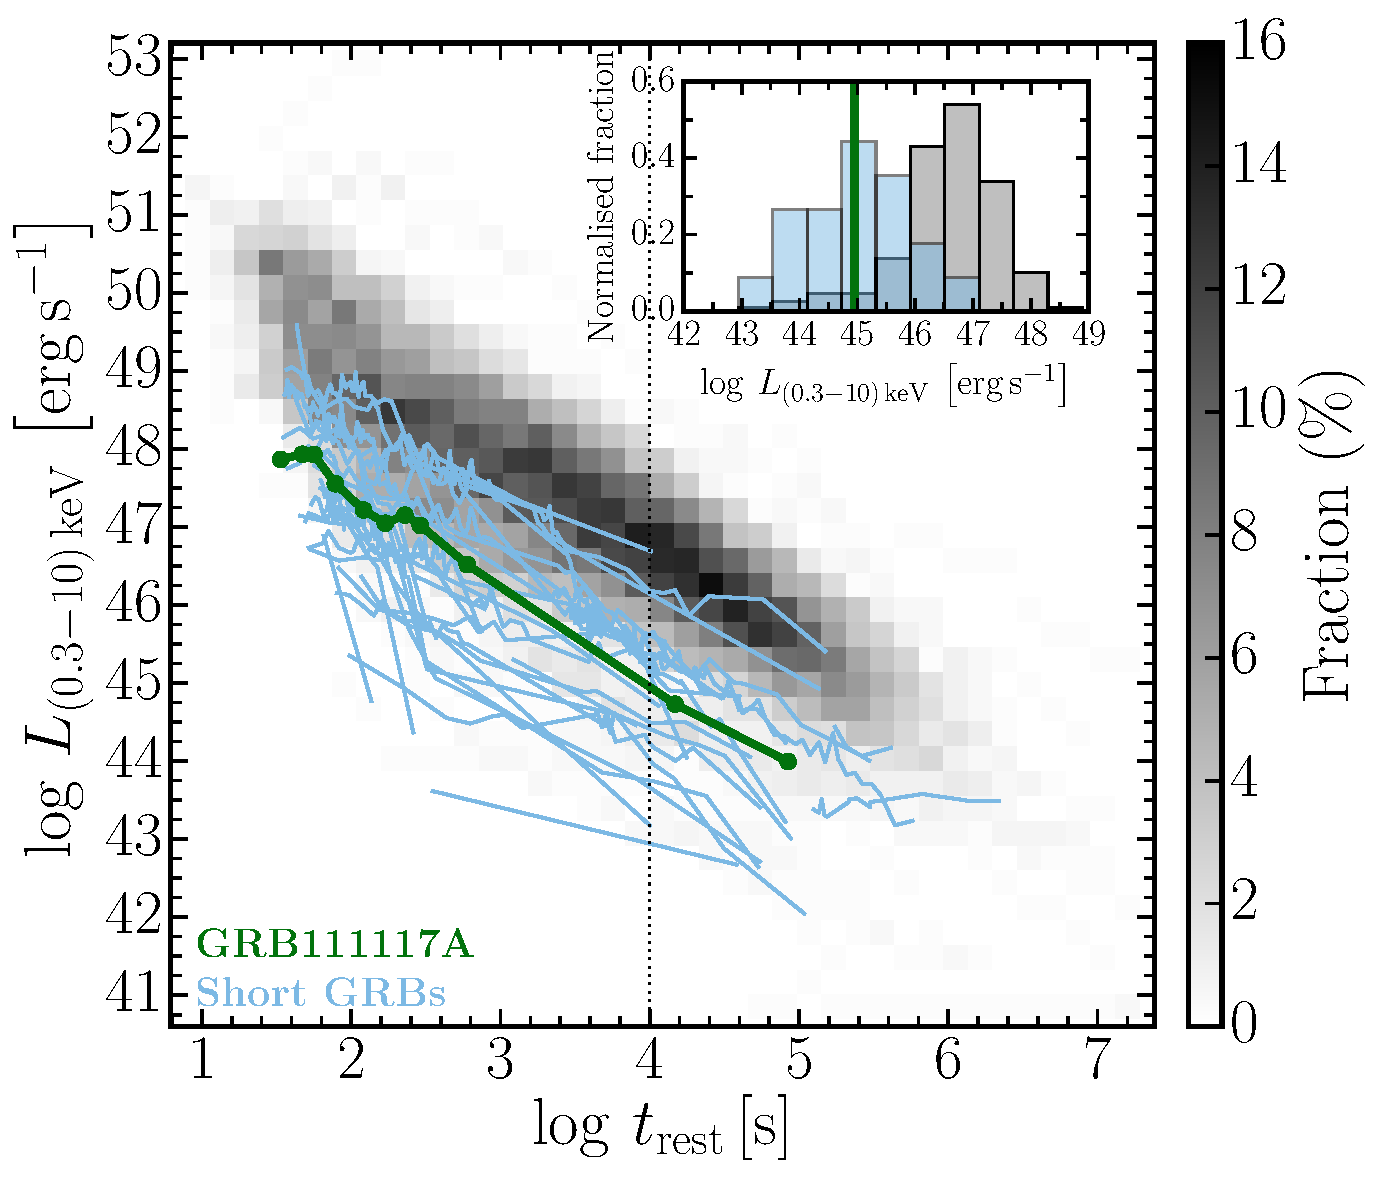
\includegraphics[width=9cm]{figures/XLC_111117A_rest.pdf}
%	\caption{Restframe XRT lightcurve of GRB~111117A, compared to the general population of XRT lightcurves of GRBs. The grey shaded region is a compilation of long GRB lightcurves from \todo{reference} where the color represents density and the light blue lines are other short GRB lightcurves from \todo{reference} for which redshifts has been determined. Despite the remarkably high redshift, the luminosity is comparable to the bulk of the short burst population and still subluminous compared to the lGRB population.}
%	\label{fig:sxray_lightcurve}
%\end{figure}

%%%%%%%%%%%%%%%%%%%%%%%%%%%%%%%%%%%%%%%%%%%%%%%%%%%%%%%%%%%%%%%%%%%%%%%%%%%%
\subsection{Restframe $N_\mathrm{H}$} \label{restnH}
%%%%%%%%%%%%%%%%%%%%%%%%%%%%%%%%%%%%%%%%%%%%%%%%%%%%%%%%%%%%%%%%%%%%%%%%%%%%

We show the recalculated $N_\mathrm{H}$ in Fig.~\ref{fig:NH_z} where we compare
with the distributions of complete samples of both long and short GRBs. The lGRB
sample is from \citet{Arcodia2016} and the sGRB sample is from
\citet{DAvanzo2014a}. 17 out of the 99 long bursts do not have redshifts, and
likewise for 5 out of 16 in the short sample. Bursts without redshifts have been
excluded for both groups. GRB~111117A occupies a unique position in
Fig.~\ref{fig:NH_z} with the highest $N_H$ of all short bursts. Additionally the
upper limit at $z = 2.609$ belongs to GRB~090426 and does not belong in the
short sample. The short sample, excluding GRB~111117A, is located at low
redshifts ($z < 1$) and is found to populate a similar column density
environment to lGRBs at similar redshifts \citep{DAvanzo2014a}. The inferred
hydrogen column for GRB~111117A seems to follow the trend with increasing $N_H$
as a function of redshift as found for the lGRB afterglows \citep{Arcodia2016}. 

%For lGRBs, $N_H$ correlates with the surface luminosity at the explosion site
%\citep{Lyman2017}, which is a challenge to reconcile  with the relatively large
%offset from the host center derived in \citet{Margutti2012} and
%\citet{Sakamoto2013}. This could suggest that there is some galaxy under the
%burst position that we don’t see. Along with the absence of dust, the large
%offset from the host center indicates that the high $N_H$ arises because the
%density in the GRB surrounding is high, or because the light from the afterglow
%traverses a region of star formation.

\begin{figure}
	\centering
	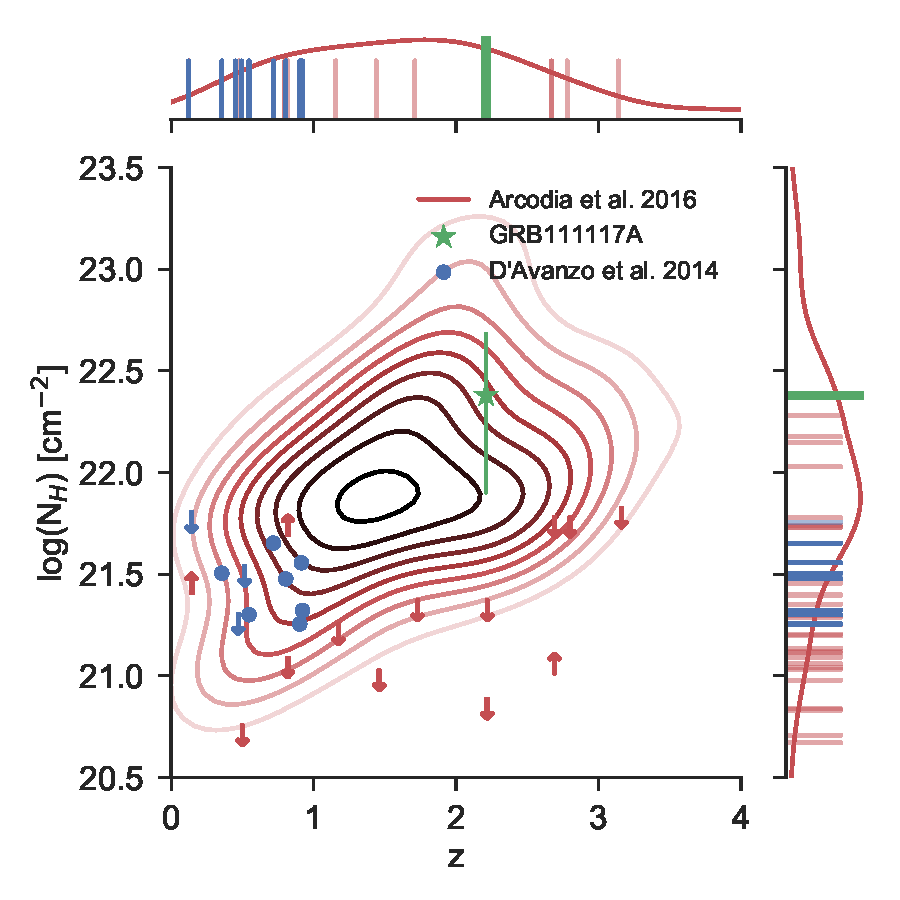
\includegraphics[width=9cm]{figures/NH_z.pdf}
	\caption{Rest frame, X-ray derived equivalent hydrogen column densities for GRB~111117A compared to complete samples of both long and short populations. The detections are replaced with contours for clarity and the limits are shown with arrows.}
	\label{fig:NH_z}
\end{figure}

% \begin{figure}
% 	\centering
% 	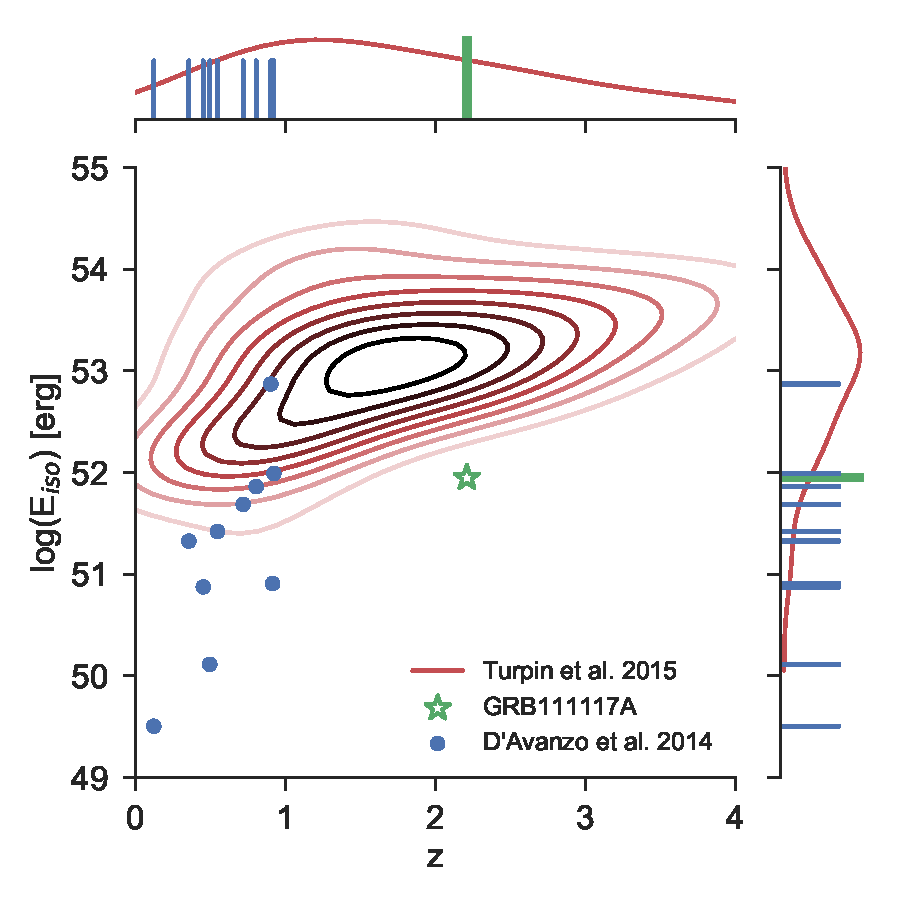
\includegraphics[width=9cm]{figures/Eiso_z.pdf}
% 	\caption{Isotropic equivalent energy for all the representative samples of both long and short GRBs. The sample is from \citet{Turpin2015} and the short is from \citet{DAvanzo2014a}.}
% 	\label{fig:NH_z}
% \end{figure}

%%%%%%%%%%%%%%%%%%%%%%%%%%%%%%%%%%%%%%%%%%%%%%%%%%%%%%%%%%%%%%%%%%%%%%%%%%%%
\subsection{Host galaxy}
%%%%%%%%%%%%%%%%%%%%%%%%%%%%%%%%%%%%%%%%%%%%%%%%%%%%%%%%%%%%%%%%%%%%%%%%%%%%

%From the clear host association, GRB~111117A does not belong to the hostless
%class of GRBs \citep{Berger2010a} and because the host exhibits emission lines
%this is indicative of a population of relatively young stars.
As the majority of sGRBs \citep{Fong2013b}, the host of GRB~111117A is a
late-type galaxy and is entirely consistent in terms of stellar mass and stellar
age with the general population of sGRB hosts ($\left\langle M _*
\right\rangle = 10^{10.1} M_{\odot}$ and $\left\langle \tau _* \right\rangle =
0.3 $~Gyr) \citep{Leibler2010}. Being a late-type host, both the stellar mass
and sSFR are entirely within the range expected for the hosts of sGRBs
\citep{Behroozi2014}. The SFR is $\sim$1 order of magnitude higher than the
typical SFR for sGRB host galaxies \citep{Berger2014} and more similar to
the SFR found in the hosts of lGRBs at a corresponding redshift
\citep{Kruhler2015}. The high SFR is partly a selection effect, because a less
star forming galaxy would exhibit weaker emission lines, thus making the
redshift harder to determine. Additionally, it is natural to expect some
evolution in the hosts of sGRBs with redshift as illustrated in Sect.~\ref{restnH}. 

%The detection of \lya~is consistent with the SED-inferred absence of dust,
%despite the moderate stellar age which would suggest the opposite. The centroid
%of the Ly$\alpha$ emission is found to be redshifted by $\sim$~220~km~s$^{-1}$
%with respect to systemic, which is similar to what is found for long GRB hosts
%\citep{Milvang-Jensen2012a} where the outflow is attributed to star formation.

%%%%%%%%%%%%%%%%%%%%%%%%%%%%%%%%%%%%%%%%%%%%%%%%%%%%%%%%%%%%%%%%%%%%%%%%%%%%%
%\subsection{Comparison to long GRBs at z $\sim$ 2}
%%%%%%%%%%%%%%%%%%%%%%%%%%%%%%%%%%%%%%%%%%%%%%%%%%%%%%%%%%%%%%%%%%%%%%%%%%%%%


%%%%%%%%%%%%%%%%%%%%%%%%%%%%%%%%%%%%%%%%%%%%%%%%%%%%%%%%%%%%%%%%%%%%%%%%%%%%
\section{Implications for the redshift distribution of sGRBs}
%%%%%%%%%%%%%%%%%%%%%%%%%%%%%%%%%%%%%%%%%%%%%%%%%%%%%%%%%%%%%%%%%%%%%%%%%%%%

A single sGRB at high redshift does little in terms of constraining the redshift
distribution of sGRBs. In particular, other sGRB hosts could be missed because
they are intrinsically fainter and thus this high-$z$ event is only detected due
to the brightness of it's host. \citet{Berger2014} compiled a sample of sGRB
host luminosities, normalized by the characteristic galaxy luminosity at their
respective redshift, $L_B/L^{\star}_{B}$. Out of the 39 hosts in the sample, 26
(66 per cent) have redshifts. To convert the SED-inferred $M_B$ of GRB~111117A
to $L_B/L^{\star}_{B}$, we use the characteristic absolute $B$-band magnitude of
the Schechter function for blue galaxies ($U - V < 0.25$) in the redshift window
$2.0 \leq z \leq 2.5$ from \citet{Marchesini2007}. For GRB~111117A, we obtain
$L_B/L^{\star}_{B} = 1.2$, which is brighter than 70 per cent of the hosts in
\citet{Berger2014} with measured $L_B/L^{\star}_{B}$.

If we assume that we are able to obtain emission-line redshifts from hosts with
$R < 25$~mag \citep{Kruhler2012}, then we would have missed around 30 per cent
(8 out of 26 from the sample of \citealt{Berger2014} with measured
$L_B/L^{\star}_{B}$), if they were at the redshift of GRB~111117A. Because the
average SFR of galaxies hosting lGRBs is higher than for galaxies hosting sGRBs,
the fraction of missed burst redshifts is likely higher although the cosmic SFR
evolution could play a role in improving redshift determinability.

A fraction of the bursts missing redshift are host-less and is therefore likely
at moderate redshifts \citep{Tunnicliffe2014}, but should some of the remainder
be at high redshift, the missed fraction will increase. If we assume that
\textit{all} the bursts that are missing redshifts in \citet{Berger2014} are at
high-$z$ and missed due to host faintness, 22 out of 39 hosts (55 per cent)
would be missed at $z = 2.211$. This serves as an upper limit on the fraction of
missed burst at high-$z$ and illustrates that we are likely \textit{not} missing a
large fraction of sGRBs redshift at $z \approx 2$ due to host faintness.

The theoretical redshift distribution of sGRBs depends on the type of delay-time
function used to model the progenitor system. The likelihood preferred lognormal
time delay models investigated by \citet{Wanderman2015} predict a sGRB rate at
$z = 2.211$, $\sim$ two orders of magnitude lower compared to the peak rate at
$z = 0.9$. According to \citet{Wanderman2015}, this preference depends
critically on the absence of non-collapsar sGRBs at $z \gtrsim 1.2$. The
redshift of GRB~111117A, on the other hand, is close to the expected peak in
sGRB rate calculated using the power law delay time models \citep{Behroozi2014,
	Wanderman2015}.


%%%%%%%%%%%%%%%%%%%%%%%%%%%%%%%%%%%%%%%%%%%%%%%%%%%%%%%%%%%%%%%%%%%%%%%%%%%
\section{Constraints on progenitor separation}
%%%%%%%%%%%%%%%%%%%%%%%%%%%%%%%%%%%%%%%%%%%%%%%%%%%%%%%%%%%%%%%%%%%%%%%%%%%

At $z = 2.211$, the age of the universe is 3 Gyr. If the progenitor systems of
sGRBs are the merger of two NSs, this sets a hard upper limit to the coalescence
timescale for such a system. In the absence of other mechanisms, the timescale
of the orbital decay of the system is set by the energy loss due to
gravitational waves, which in turn is set by the mass of the constituent compact
objects and the separation of the two \citep{Postnov2014}. If we assume that the
formation timescale of the first galaxies is short compared to the time since
the Big Bang \citep{Richard2011}, and if we assume a mass of 1.4~$M_\odot$ for
each of the NSs at the time of system formation, this places a hard upper limit
on the initial separation, of $a_0 < 3.2~R_\odot$.

In practice most NS-NS binaries will be eccentric at formation because of the SN
natal kicks, and this can be quite a big effect on merger times, although
eccentric systems normally circularise first. It could also be a BH-NS system,
and as the merger time scales roughly as $M^3$ the mass here almost as big an
effect as the separation ($a^4$).

Using the inferred stellar population age from our SED fit, then we obtain a
(softer) limit on the initial separation of $a_0 < 2.1~R_\odot$. However, this
does not account for the possibility there could be an underlying stellar
population of older stars from a previous star-formation epoch. The delay time
between formation and explosion is well accommodated by the models of
\citet{Belczynski2006}, although the longest delay times are excluded.
This is especially true given the late type nature of the host
\citep{OShaughnessy2008}.

%%%%%%%%%%%%%%%%%%%%%%%%%%%%%%%%%%%%%%%%%%%%%%%%%%%%%%%%%%%%%%%%%%%%%%%%%%%%
\section{Conclusions}
%%%%%%%%%%%%%%%%%%%%%%%%%%%%%%%%%%%%%%%%%%%%%%%%%%%%%%%%%%%%%%%%%%%%%%%%%%%%

In this \emph{Letter}, we have provided a revised, spectroscopic redshift for
the short GRB~111117A based on emission lines setting it at $z = 2.211$. This
value supersedes the previous photometric redshift of \citet{Margutti2012} and
\citet{Sakamoto2013}. %The erroneous redshift estimate of previous authors is
%attributed to a discrepancy in the measured $z$-band magnitude.

Using the new distance, the X-ray derived $n_H$ towards GRB~111117A is the
highest within a complete sample of sGRB hosts and is consistent with the
$n_H-z$ evolution traced by the hosts of lGRBs.The SFR of the host is in the
upper end of the sGRB host SFR distribution and no dust is present. The high
$N_H$ is difficult to reconcile with the large projected host offset and the
absence of dust. One possible explanation could be, that GRB~111117A is formed
through the prompt channel of sGRBs \todo{ref} and originates in a star forming
region located in the outskirts of the host.

Although a single burst carries little leverage in terms of constraining the
redshift distribution of sGRB, the high redshift of GRB~111117A needs to be
accommodated in progenitor models. A lognormal delay time model predicts a very low volumetric
density of bursts at $z = 2.211$, whereas a power law delay time model peaks
near GRB~111117A. If more sGRBs are at similarly high redshifts, but are missed due to
the faintness of their hosts, a lognormal delay time model will be disfavored.
Compared to a sample of sGRB hosts, GRB~111117A is more luminous than 70 per
cent of the sample with measured luminosities. Conservatively, for 55 per
cent of the sGRB hosts, we would be unable to determine a redshift should they be at 
a similar redshift as GRB~111117A. This implies that we are \textit{not} missing a large
fraction of the sGRBs at $z \sim 2$.

Using the age of the universe at the time of explosion allows us to set
constraints on the maximal separation between the engine constituents at the
time of formation. We find that the maximal separation of two NSs at
formation time is $a_0 < 3.2~R_\odot$, which excludes some of the formation
channels with the longest timescales.

All data, code and calculation related to the paper along with the
paper itself are available at \url{https://github.com/jselsing/GRB111117A}.

\begin{acknowledgements}
TK acknowledges support through the Sofja Kovalevskaja Award to P. Schady. 
CT acknowledges support from a Spanish National Research Grant of Excellence under project AYA 2014-58381-P and funding associated to a Ramón y Cajál fellowship under grant number RyC-2012-09984.
AdUP acknowledges support from a Ramón y Cajal fellowship, a BBVA Foundation Grant for Researchers and Cultural Creators,and the Spanish Ministry of Economy and Competitiveness through project AYA2014-58381-P.
Partly based on observations made with the Gran Telescopio Canarias (GTC).
ZC acknowledges support from the Spanish research project AYA 2014-58381-P and support from Juan de la Cierva Incorporaci\'on fellowships IJCI-2014-21669. 

\end{acknowledgements}

\bibliographystyle{mnras}
\bibliography{GRB111117A}

\newpage
%\appendix

\input{tables/spec_overview.tex}

\begin{table*}[!ht]

	\centering
	\caption{Overview of the photometric observations. \label{tab:phot_overview}}
	\begin{tabular}{ccccccc}
		\hline\hline
{Obs. Date} &  Exptime & Telescope/Instrument & Filter & Airmass & Image Quality & Host Brightness\tablefootmark{a}  \\ [1.5pt]
        \hline
{} & {ks} &    & {} & & (arcsec)  & (mag$_{\mathrm{AB}}$)  \\ [1.5pt]
		\hline
2013-08-30T07:43 & 1.45 & VLT/FORS2 & $g$ & 1.55 & 0.99 & $24.08\pm 0.09$ \\
2011-11-17T20:07 & 0.80 & GTC/OSIRIS & $g$ & 1.15 & 1.67 & $24.13\pm 0.09$ \\
2011-11-17T20:07 & 1.20 & GTC/OSIRIS & $r$ & 1.11 & 1.50 & $23.93\pm 0.08$ \\        
2013-07-17T08:37 & 1.45 & VLT/FORS2 & $R$ & 1.56 & 0.74 & $23.95\pm 0.06$ \\   
2011-11-28T21:10 & 3.60 & TNG/DOLORES & $R$ & 1.01 & 1.08 & $23.96\pm 0.13$ \\           
2011-11-17T20:07 & 0.36 & GTC/OSIRIS & $i$ & 1.08 & 1.50 & $23.89\pm 0.23$ \\   
2013-08-03T09:23 & 1.35 & VLT/FORS2 & $I$ & 1.54 & 0.93 & $24.22\pm 0.15$ \\           
2011-11-28T06:14 & 1.80 & Gemini/GMOS-N & $z$ & 1.01 & 0.84 & $24.24\pm 0.47$ \\  
2013-07-13T09:33 & 1.08 & VLT/FORS2 & $z$ & 1.49 & 0.63 & $23.76\pm 0.21$ \\             
2013-06-24T09:14 & 1.98 & VLT/HAWK-I & $J$ & 1.70 & 0.63 & $23.13\pm 0.18$ \\        
2013-06-27T09:21 & 1.68 & VLT/HAWK-I & $H$ & 1.63 & 0.91 & $22.94\pm 0.29$ \\   
2013-06-28T09:14 & 1.92 & VLT/HAWK-I & $K_\mathrm{s}$ & 1.65 & 0.76 & $23.07\pm 0.32$ \\   
\hline\noalign{\smallskip}
		
\end{tabular}

\tablefoot{
\tablefoottext{a}{All magnitudes are given in the AB system and are not corrected for the expected Galactic foreground extinction corresponding to a reddening of $E_{B-V}=0.027$\,mag.}}
\end{table*}

 \begin{figure*}
 	\centering
 	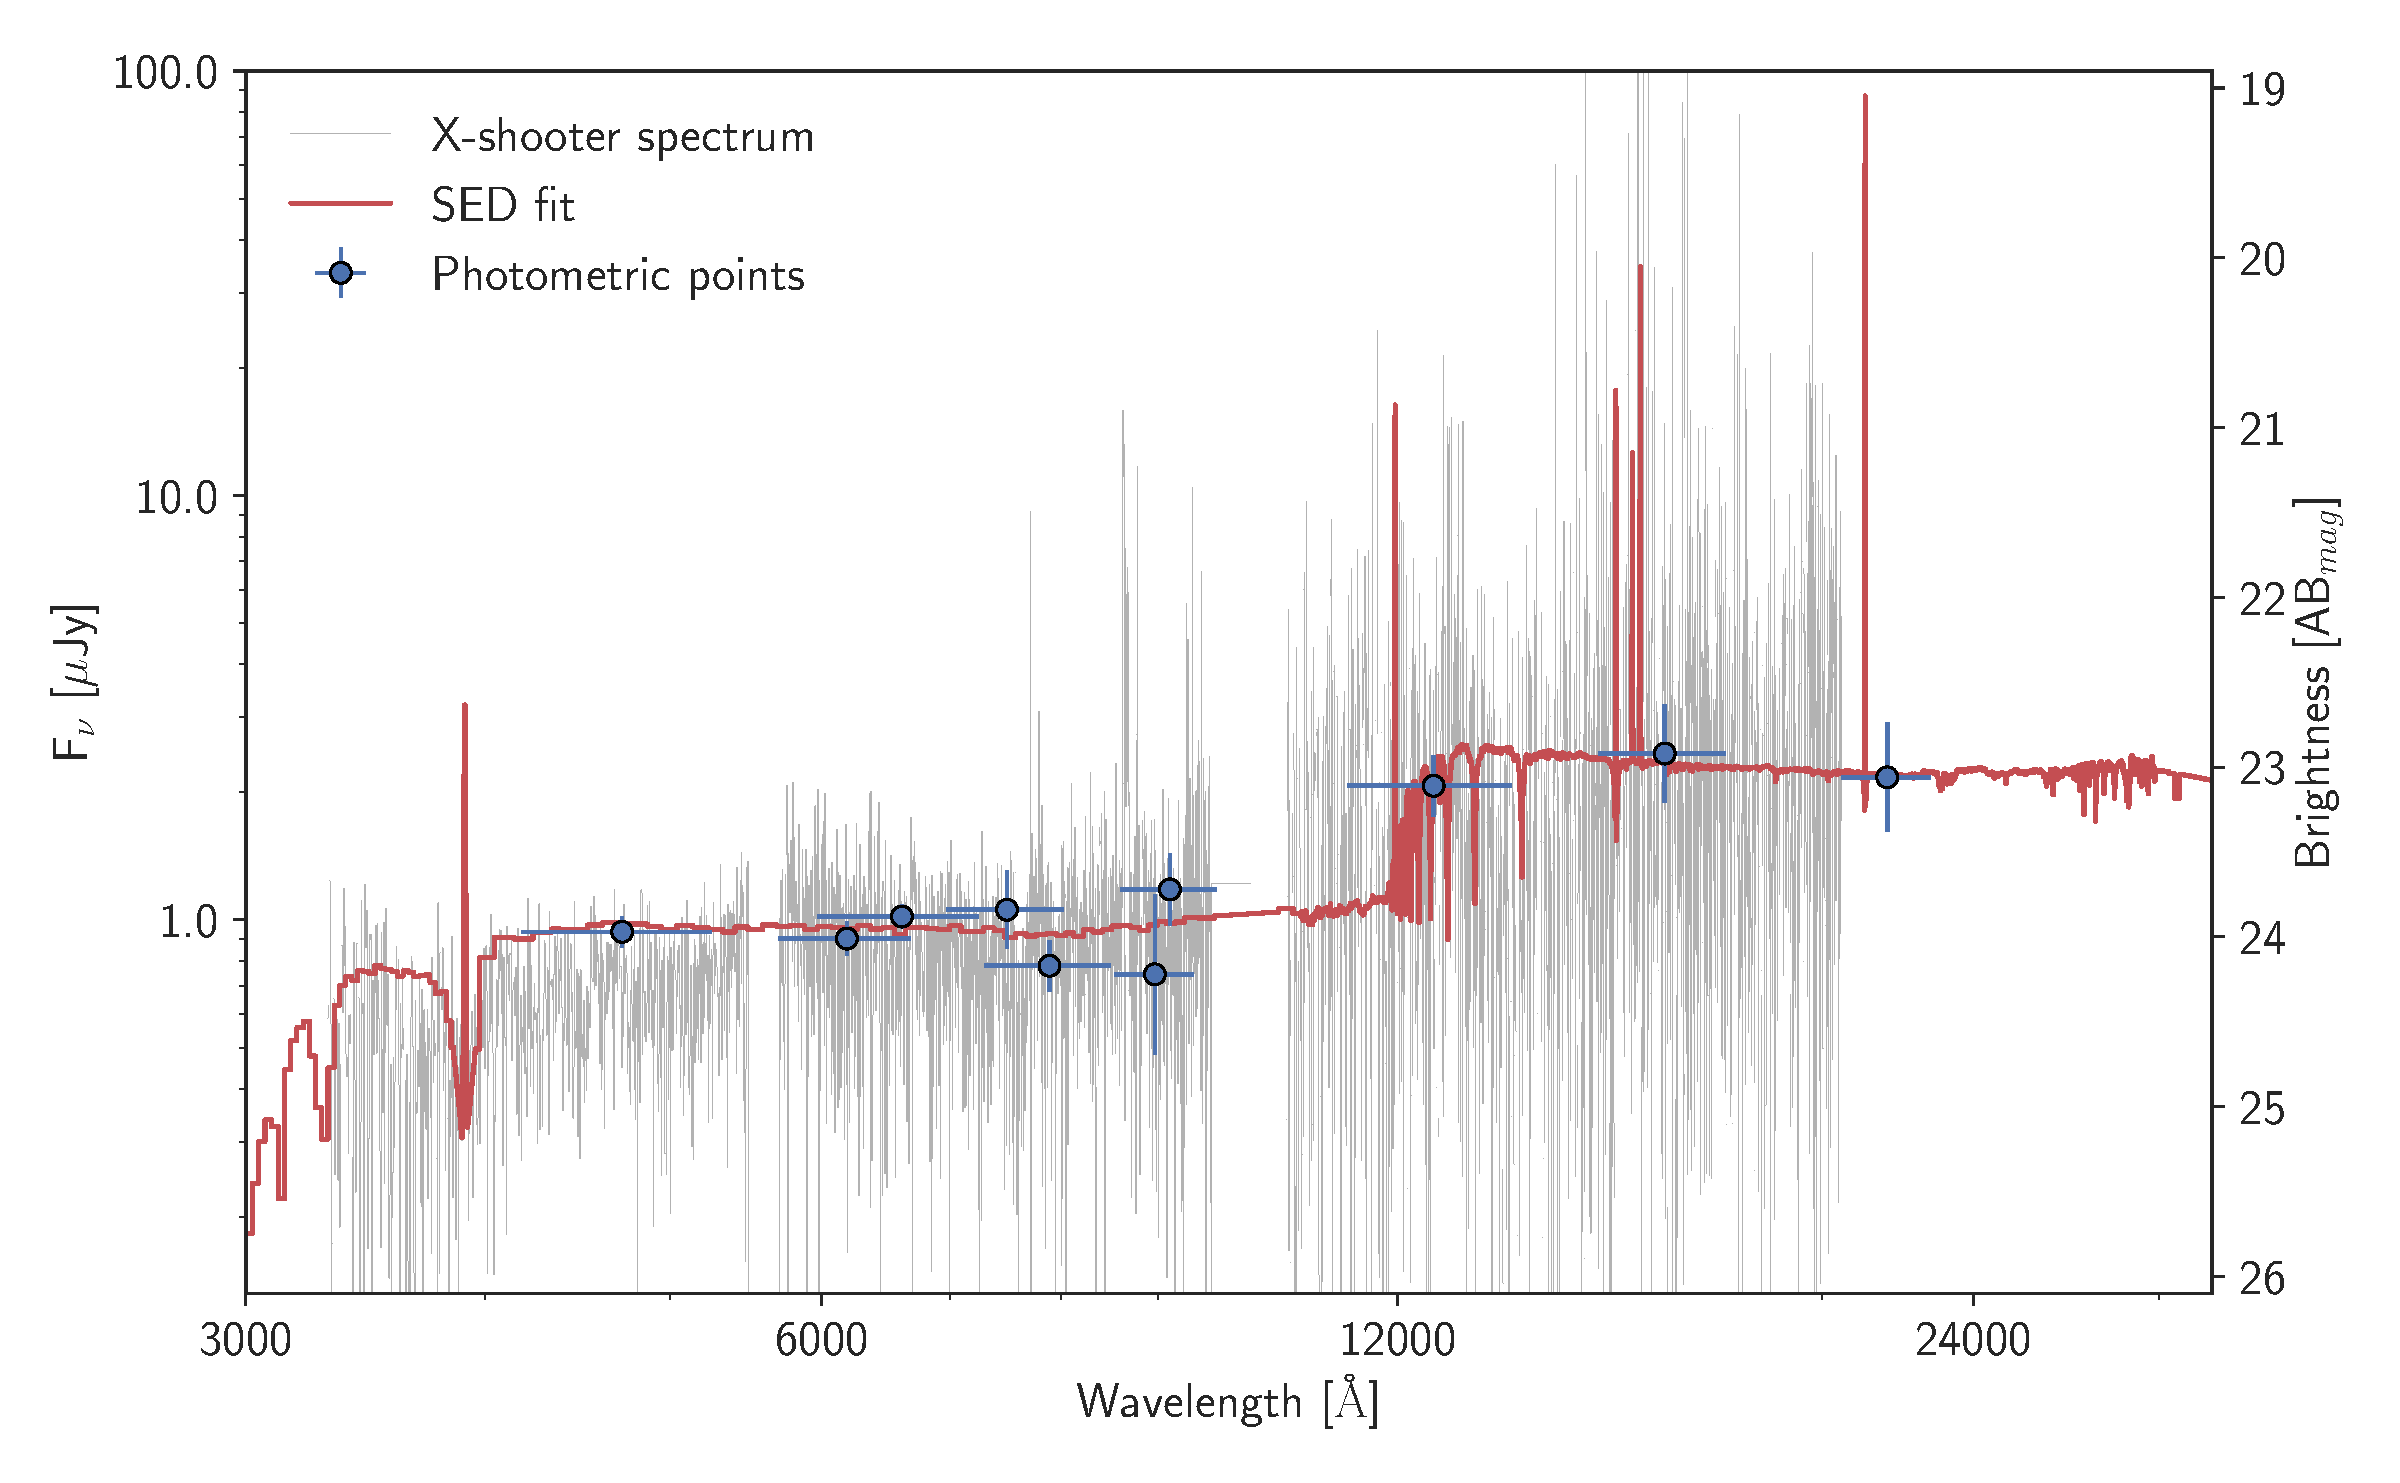
\includegraphics[width=16cm]{figures/SEDspecphot.pdf}
 	\caption{SED fit showning the best-fist SED to the derived photometry. The detection of \lya~ is predicted from the SED fit and confirmed by the spectroscopic observations. Overplotted in grey is the observed spectrum. The reason for the spectral gaps at 5500 \AA~and 10000 \AA~is from the merging of the arms.}
 	\label{fig:SED}
 \end{figure*}



\end{document}


